\documentclass{beamer}
\usepackage[utf8]{inputenc}  % 输入字符集为UTF-8
\usepackage{ctex}  % 支持中文
\usepackage{amsmath}  % 支持数学符号
\usepackage{hyperref}  % 支持超链接
\usepackage{graphicx}  % 插入图片

\title{动态规划背包模型 + 线性 DP}
\author{}
\date{}

\begin{document}

\frame{\titlepage}

\section{什么是dp?}

\begin{frame}{DP(Dynamic programming) 既动态规划问题}
    动态规划是一种将一个复杂问题分解为多个简单的子问题求解的方法。将子问题的答案存储在记忆数据结构中,当子问题再次需要解决时,只需查表查看结果,而不需要再次重复计算,因此节约了计算时间。
\end{frame}

\section{动态规划基本概念}

\begin{frame}{最优子结构}
    最优子结构是动态规划问题的一个重要特征。它意味着一个最优解可以由其子问题的最优解构成。换句话说,如果我们能够找到子问题的最优解,那么就可以通过组合这些子问题的解来构建原问题的最优解。
\end{frame}

\begin{frame}{重叠子问题}
    重叠子问题指的是在求解一个问题的过程中,需要多次求解一些相同的子问题。如果我们能够将这些子问题的解存储起来,就可以避免重复计算,从而提高效率。
\end{frame}

\begin{frame}{状态转移方程}
    状态转移方程是动态规划的核心,它描述了当前状态与之前状态之间的关系。通过状态转移方程,我们可以将一个复杂的问题分解为更简单的子问题,并利用子问题的解来构建原问题的解。
\end{frame}

\begin{frame}{记忆化搜索}
    记忆化搜索是动态规划的一种实现方式。它通过维护一个存储结构(如哈希表或数组)来记录已经计算过的子问题的解,从而避免重复计算。当需要求解一个子问题时,首先检查它是否已经被计算过,如果是,直接返回存储的结果;否则,计算该子问题的解并将其存储起来。
\end{frame}

\section{常见dp问题}

\begin{frame}{常见dp问题}
    \begin{itemize}
        \item 线性 DP
        \item 区间 DP
        \item 背包 DP
        \item 树形 DP
        \item 状态压缩 DP
        \item 数位 DP
        \item 计数型 DP
        \item 递推型 DP
        \item 概率型 DP
        \item 博弈型 DP
        \item 记忆化搜索
    \end{itemize}
\end{frame}

\section{线性dp基础}

\begin{frame}{线性dp的特点}
    线性dp的特点是其状态转移存在一个线性关系。
\end{frame}

\begin{frame}{斐波那契数列 (洛谷B2064)}
    斐波那契数列是指这样的数列:数列的第一个和第二个数都为 $1$,接下来每个数都等于前面 $2$ 个数之和。给出一个正整数 $a$,要求斐波那契数列中第 $a$ 个数是多少。
\end{frame}

\begin{frame}{最长上升子序列(洛谷B3637)}
    给出一个由 $n(n\le 5000)$ 个不超过 $10^6$ 的正整数组成的序列。请输出这个序列的\textbf{最长上升子序列}的长度。最长上升子序列是指,从原序列中\textbf{按顺序}取出一些数字排在一起,这些数字是\textbf{逐渐增大}的。
\end{frame}

\begin{frame}{数字三角形(洛谷P1216)}
    观察下面的数字金字塔。写一个程序来查找从最高点到底部任意处结束的路径,使路径经过数字的和最大。每一步可以走到左下方的点也可以到达右下方的点。
    \begin{figure}
        \centering
        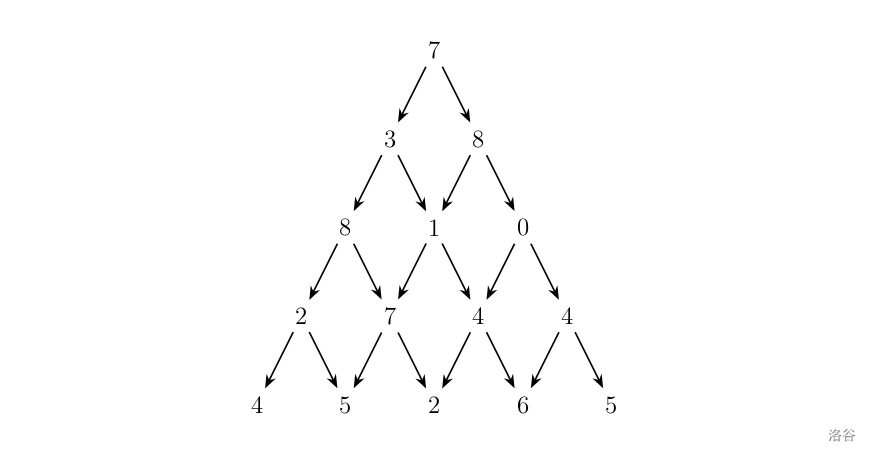
\includegraphics[width=0.5\textwidth]{./ex.png}
    \end{figure}
    在上面的样例中,从 $7 \rightarrow 3 \rightarrow 8 \rightarrow 7 \rightarrow 5$ 的路径产生了最大权值。
\end{frame}

\begin{frame}{最长公共子序列(洛谷P1439)}
    给出 $1,2,\ldots,n$ 的两个排列 $P_1$ 和 $P_2$ ,求它们的最长公共子序列。
    \begin{itemize}
        \item 最长上升子序列的元素不一定相邻。
        \item 最长上升子序列一定是原序列的子集。
    \end{itemize}
\end{frame}

\begin{frame}{编辑距离 (P2758)}
    设 $A$ 和 $B$ 是两个字符串。我们要用最少的字符操作次数,将字符串 $A$ 转换为字符串 $B$。这里所说的字符操作共有三种:
    \begin{itemize}
        \item 删除一个字符;
        \item 插入一个字符;
        \item 将一个字符改为另一个字符。
    \end{itemize}
    $A, B$ 均只包含小写字母。
\end{frame}

\section{背包问题}

\begin{frame}{01背包}
    有n件物品和一个最多能背重量为w 的背包。第i件物品的重量是$weight[i]$,得到的价值是$value[i]$。每件物品只能用一次,求解将哪些物品装入背包里物品价值总和最大。
\end{frame}

\begin{frame}{贪心选择策略不适用于0-1背包问题}
    对于0-1背包问题,贪心选择之所以不能得到最优解是因为,在这种情况下,它无法保证最终能将背包装满,部分闲置的背包空间使每千克背包空间的价值降低了。 事实上,在考虑0-1背包问题时,应比较选择该物品和不选择该物品所导致的最终方案,在做出最好选择。由此可导出许多互相重叠的子问题。这正是该问题可用动态规划算法求解的另一重要特征。
\end{frame}

\begin{frame}{完全背包}
    有N件物品和一个最多能背重量为W的背包。第i件物品的重量是$weight[i]$,得到的价值是$value[i]$。每件物品都有无限个(也就是可以放入背包多次),求解将哪些物品装入背包里物品价值总和最大。
\end{frame}

\begin{frame}{多重背包}
    有N件物品和一个最多能背重量为W的背包。第i件物品的重量是$weight[i]$,得到的价值是$value[i]$。对于每件物品i都有$a[i]$个(也就是可以放入背包a[i]次),求解将哪些物品装入背包里物品价值总和最大。
\end{frame}

\begin{frame}{分组背包}
    有n件物品和一个最多能背重量为w 的背包。将n件物品分为m组,每组物品有若干个,同一组内的物品最多只能选一个。第i件物品的重量是$weight[i]$,得到的价值是$value[i]$。每件物品只能用一次,求解将哪些物品装入背包里物品价值总和最大。
\end{frame}

\end{document}
